% \chapter{Preliminaries} 
% \label{ch:prelim}



% \begin{chapternotes}
%   This chapter contains material previously published ...
% \end{chapternotes}

\section{Beispiel-Inhalte}
Dieser Abschnitt zeigt beispielhaft, wie man Inhalte wie Grafiken, Tabellen, Quelltext, Referenzen etc. einfügt. 

\subsection{Grafiken}
Eine Grafik liegt üblicherweise in einer fließenden \texttt{figure}-Umgebung und wird mittels \verb+\includegraphics+ eingebunden, siehe \autoref{fig:example}.

\begin{figure}
	\centering
	\includegraphics[width=3cm]{htl_at}
	\caption{Example caption.}
	\label{fig:example}
\end{figure}

Mit Hilfe des Pakets \emph{TikZ} können auch Grafiken direkt in \LaTeX erstellt werden, siehe \zB \autoref{fig:def:prelim:ltl:kl-loop} auf Seite~\pageref{fig:def:prelim:ltl:kl-loop}.

\begin{figure}
  \centering
  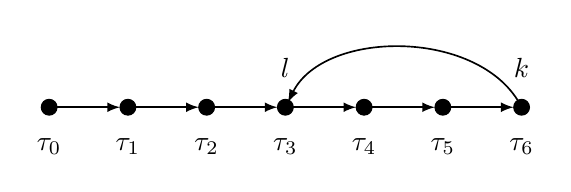
\begin{tikzpicture}
    \foreach \x in {0,1,2,3,4,5,6} 
    \draw[fill] (\x,5.5) circle (0.1);
    \foreach \x in {0,1,2,3,4,5} 
    \draw[-latex,semithick] (\x,5.5) -- +(0.9,0);
    \draw[-latex,shorten >=2,semithick] (6,5.5) .. controls (5.5,6.5) and (3.5,6.5) .. (3,5.5);
    \foreach \x in {0,1,2,3,4,5,6}
    \node at (\x,5) {$\tau_{\x}$};
    % \node at (-0.5,5) {$t=$};
    \node at (6,6) {$k$};
    \node at (3,6) {$l$};
  \end{tikzpicture}
  \caption{Some funny picture}
  \label{fig:def:prelim:ltl:kl-loop}
\end{figure}

\subsection{Referenzen}

Referenzen werden in einer Datenbank abgelegt (hier unter {\ttfamily 99--references.bib}) und dann im Text wie folgt referenziert \cite{Bringhurst1993}. \textcite{Bringhurst1993} schrieb die "`Bibel der Typografie"'. 

\subsection{Abkürzungen}

Abkürzungen müssen in wissenschaftlichen Texten bei der ersten Verwendung definiert (erklärt). Dies wird hier durch den Befehl \verb+\ac+ erledigt. 

Beispiel: Der Begriff \ac{LTL} wurde soeben definiert und bei der weiteren Verwendung von \ac{LTL} wird nurnoch die Abkürzung ausgegeben. Die Definitionen liegen zentral in der Datei \verb+acronyms.tex+. 

\subsection{Aufzählungen und Aufzählungspunkte}
Nummerierte Aufzählungen:
\begin{enumerate}
	\item Foo
    	\begin{enumerate}
        	\item kann auch 
        	\item verschachtelt werden
        \end{enumerate}
	\item Bar
\end{enumerate}

Nicht nummerierte Aufzählungen:
\begin{itemize}
	\item One
	\item Two
	\item Three
\end{itemize}

\subsection{Tabellen}
Eine Tabelle wie jene in \autoref{tab:example} 
kann etwas einfacher mittels \url{http://www.tablesgenerator.com} erstellt werden. 

Hinweise:
\begin{itemize}
    \item Tabellen werden normalerweise oben beschriftet. 
    \item Aus typografischer Sicht sind vertikale Linien in Tabellen "`schlechter Stil"', die Spalten sollten aufgrund der Abstände erkennbar sein. 
\end{itemize}

\begin{table}
	\centering
	\caption{Beispiel für eine Tabelle}
	\label{tab:example}
	\begin{tabular}{llc}
	\toprule
	A & B & C\\
	\midrule
	1 & 2 & unknown\\
	x & y & z\\
	\bottomrule
	\end{tabular}
\end{table}

\subsection{ToDo-Notizen}

\begin{todobox}
ToDo: Diplomarbeit mit sinnvollen Inhalten füllen. 
\end{todobox}

\subsection{Quellcode-Listings}

Listings möglichst nicht als Screenshot einbinden (verpixeln, nicht änderbar, kein Seitenumbruch möglich,~\ldots), siehe \autoref{lst:java}. 

Weitere Hinweise siehe \zB \url{https://www.overleaf.com/learn/latex/Algorithms#Listings_package}. 

\begin{lstlisting}[style=text,language=Java,label=lst:java,caption={Java Code Example}]
@FacesConverter(forClass = Fraction.class)
public class FractionConverter implements Converter {
    @Override
    public Object getAsObject(FacesContext context,
            UIComponent component, String value) {
        try {
            // split at the first slash
            String[] parts = value.split("/");
            return new Fraction(Integer.valueOf(parts[0]),
                    Integer.valueOf(parts[1]));
        } catch (NumberFormatException | IndexOutOfBoundsException e) {
            throw new ConverterException(
                    new FacesMessage(FacesMessage.SEVERITY_ERROR,
                            "Not a valid fraction!", null));
        }
    }
    @Override
    public String getAsString(FacesContext context,
            UIComponent component, Object value) {
        return ((Fraction) value).toString();
    }

}
\end{lstlisting}
